
%(BEGIN_QUESTION)
% Copyright 2015, Tony R. Kuphaldt, released under the Creative Commons Attribution License (v 1.0)
% This means you may do almost anything with this work of mine, so long as you give me proper credit

Beregn utgangsspenningen i denne op-amp-kretsen gitt inngangsprofilen i grafen. Anta startladning på kondensator ($V_0$) lik +8 V:

$$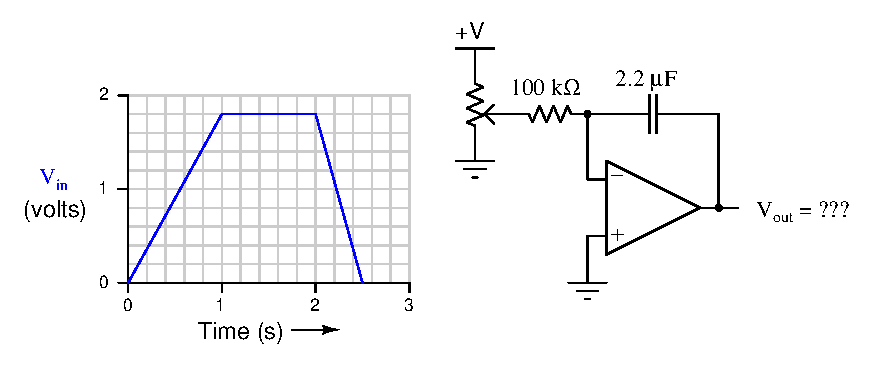
\includegraphics[width=15.5cm]{i01027x01.eps}$$

Beregn også tidskonstanten til integratorkretsen.

\underbar{file i01027}
%(END_QUESTION)





%(BEGIN_ANSWER)

$$V_{out} = -{1 \over RC} \int_{t_0}^{t_f} V_{in} \> dt + V_0$$

$$V_{out} = -\left({1 \over (100 \times 10^3 \> \Omega)(2.2 \times 10^{-6} \hbox{ F})}\right) \left( \int_{0}^{2.5} V_{in} \> dt \right) + 8 \hbox{ V}$$

Integralet finnes grafisk som arealet av trapeset i figuren.

$$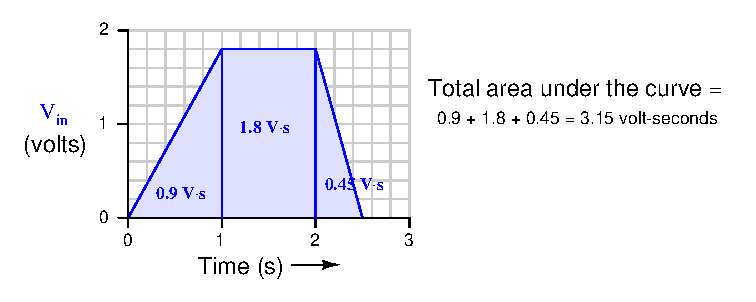
\includegraphics[width=15.5cm]{i01027x02.eps}$$

$$V_{out} = -6.318 \hbox{ V}$$

\vskip 10pt

Tidskonstant:

$$\tau_i = RC = (100 \times 10^3 \> \Omega)(2.2 \times 10^{-6} \hbox{ F}) = 0.22 \hbox{ s}$$

%(END_ANSWER)





%(BEGIN_NOTES)


%INDEX% Electronics review: integrator circuit

%(END_NOTES)

